\chapter{कोशिका, जीवन की इकाई}\label{ch:g6:cell-unit-of-life}

\Cref{ch:g5:first-look-at-cells} एक वादे पर ख़त्म हुआ था: वे छोटी
कोठरियाँ ख़ाली नहीं हैं। इस साल स्कूल का \omterm{def:g5:first-look-at-cells:microscope}{सूक्ष्मदर्शी} फिर बाहर आता है
--- बेहतर स्लाइडों और पैने सवालों के साथ। \omterm{def:g5:first-look-at-cells:cell}{कोशिका} में ठीक-ठीक क्या होता
है? क्या \omterm{def:g1:plants-around-us:plant}{पौधे} और \omterm{def:g1:animals-around-us:animal}{जंतु} की \omterm{def:g5:first-look-at-cells:cell}{कोशिकाएँ} अलग होती हैं? और क्या \omterm{def:g5:first-look-at-cells:cell}{कोशिका} जीवन का
कोई \emph{हिस्सा} है, या एक \omterm{def:g5:first-look-at-cells:cell}{कोशिका} पूरा \omterm{def:g6:exploring-our-environment:components}{सजीव} भी हो सकती है?
\omterm{def:g1:living-or-not:living}{जीवविज्ञान} की सबसे छोटी इकाई एक पूरे अध्याय की हक़दार है।

\section{कोशिका के भीतर}

\begin{definition}[कोशिका के भाग]\label{def:g6:cell-unit-of-life:parts}
ठीक से देखो तो हर \omterm{def:g5:first-look-at-cells:cell}{कोशिका} वही बुनियादी साज़-सामान दिखाती है:
\begin{enumerate}
  \item \emph{झिल्ली}\index{झिल्ली}, यानी \omterm{def:g5:first-look-at-cells:cell}{कोशिका} का पतला बाहरी लिफ़ाफ़ा,
        जो उसे बाँधे रखता है और यह क़ाबू में रखता है कि क्या भीतर आए और
        क्या बाहर जाए;
  \item \emph{कोशिकाद्रव्य}\index{कोशिकाद्रव्य}, यानी वह लसलसा भराव
        जिसमें \omterm{def:g5:first-look-at-cells:cell}{कोशिका} का काम चलता है;
  \item \emph{केंद्रक}\index{केंद्रक}
        (\cref{rem:g5:first-look-at-cells:nucleus} वाला गहरा धब्बा),
        यानी वह कमान-केंद्र जो \omterm{def:g5:first-look-at-cells:cell}{कोशिका} के जीवन और उसके विभाजन को चलाता
        है।
\end{enumerate}
झिल्ली, कोशिकाद्रव्य, केंद्रक: हर \omterm{def:g1:plants-around-us:plant}{पौधे}, हर \omterm{def:g1:animals-around-us:animal}{जंतु} और हर \omterm{def:g6:decomposers-and-soil:decomposers}{कवक} की लगभग हर
\omterm{def:g5:first-look-at-cells:cell}{कोशिका} का यही तीन हिस्सों वाला सामान है।
\end{definition}

\begin{proposition}[पौधों की कोशिकाओं में कुछ और भी होता है]\label{prop:g6:cell-unit-of-life:plantextras}
\omterm{def:g1:plants-around-us:plant}{पौधों} की \omterm{def:g5:first-look-at-cells:cell}{कोशिकाएँ} अपना कुछ साज़-सामान और जोड़ लेती हैं:
\begin{itemize}
  \item \omterm{def:g6:cell-unit-of-life:parts}{झिल्ली} के बाहर एक सख़्त \emph{कोशिका भित्ति}\index{कोशिका
        भित्ति} --- वही भित्तियाँ जो प्याज़ की \omterm{def:g6:cell-unit-of-life:parts}{झिल्ली} की ईंट-जैसी
        बनावट बनाती हैं (\cref{ex:g5:first-look-at-cells:classics})
        और \omterm{def:g1:plants-around-us:plant}{पौधों} को \omterm{def:g3:bones-and-muscles:skeleton}{हड्डियों} के बिना ही खड़े रहने की अकड़ देती हैं;
  \item \omterm{def:g6:cell-unit-of-life:parts}{कोशिकाद्रव्य} में \omterm{def:g6:exploring-our-environment:conditions}{प्रकाश} पकड़ने वाले पदार्थ के हरे कण --- यानी
        \omterm{def:g5:food-webs:roles}{उत्पादकों} की कार्यशालाएँ
        (\cref{prop:g6:plants-are-producers:produce}), जो हर \omterm{def:g1:animals-around-us:animal}{जंतु}
        \omterm{def:g5:first-look-at-cells:cell}{कोशिका} में ग़ैरहाज़िर हैं;
  \item और अकसर पानी से भरी एक बड़ी थैली, जिसका दबाव \omterm{def:g5:first-look-at-cells:cell}{कोशिका} को फूली
        हुई रखता है --- मुरझाना
        (\cref{ex:g1:plants-around-us:wilt}) इन्हीं थैलियों का ढीला
        पड़ जाना है।
\end{itemize}
\end{proposition}
\admitted

\begin{omfigure}
\begin{minipage}[t]{0.48\linewidth}\centering
\begin{tikzpicture}
  \node[anchor=south west, inner sep=0] (img) at (0,0)
    {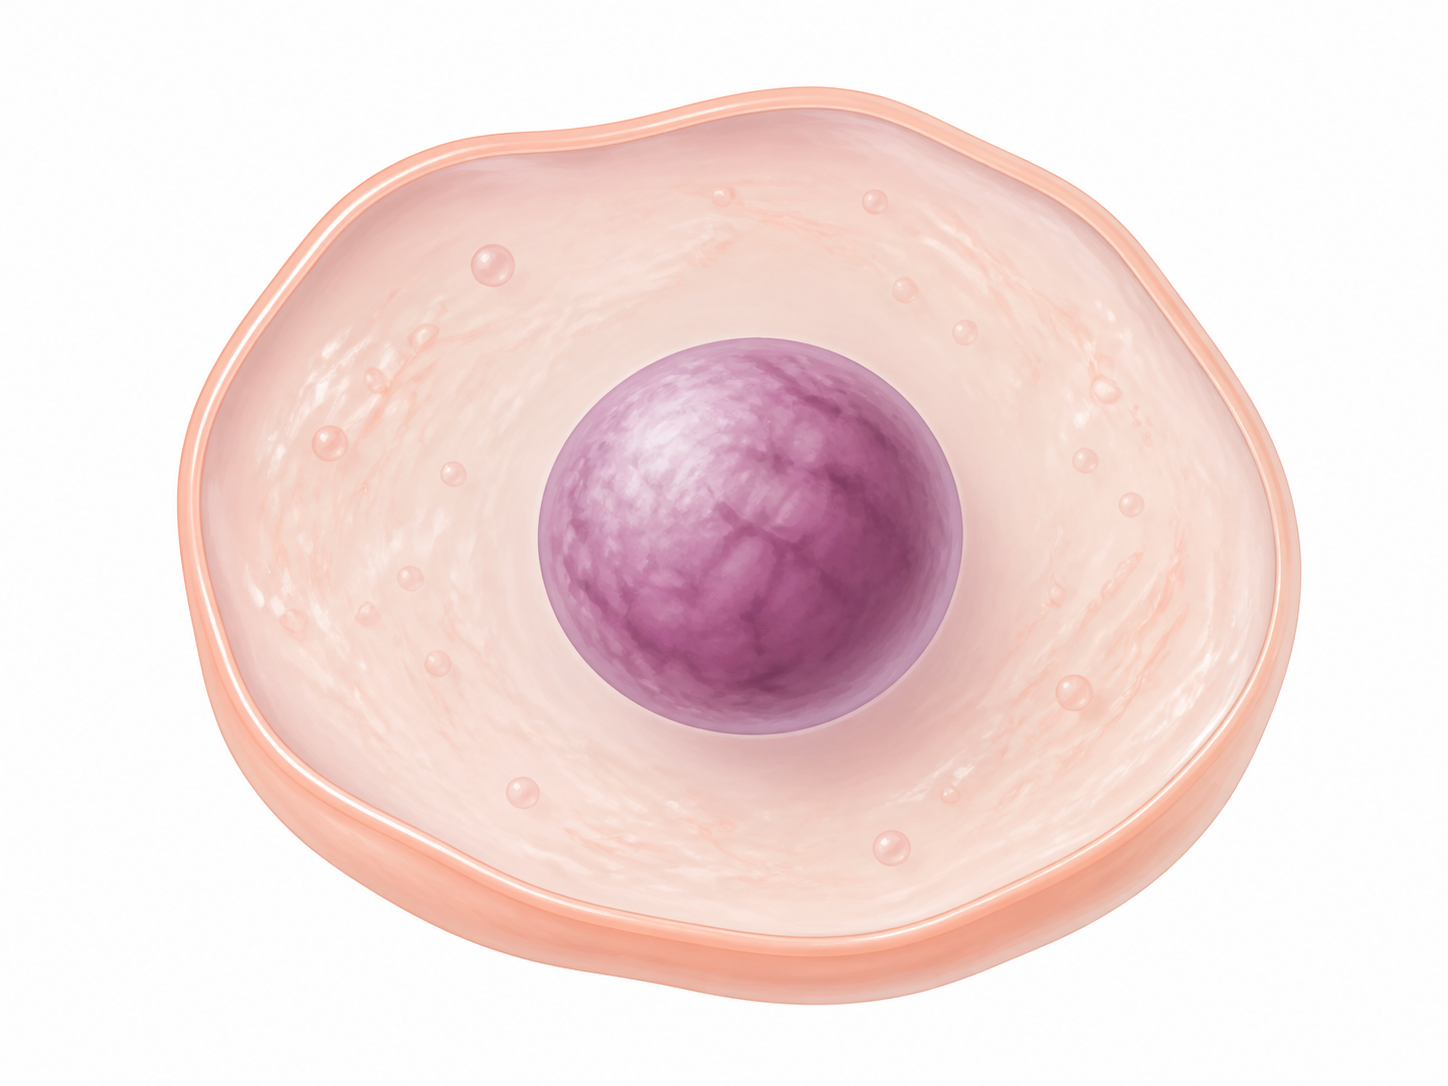
\includegraphics[width=0.9\linewidth]{images/book1/ai/fig-animal-cell.png}};
  \begin{scope}[x={(img.south east)}, y={(img.north west)},
      every node/.style={font=\footnotesize}]
    \draw[omDef, thick] (0.24,0.79) -- (0.12,0.93) node[above] {झिल्ली};
    \draw[omDef, thick] (0.32,0.42) -- (0.15,0.20)
      node[below] {कोशिकाद्रव्य};
    \draw[omDef, thick] (0.58,0.52) -- (0.80,0.20)
      node[below] {केंद्रक};
  \end{scope}
\end{tikzpicture}

{\small \omterm{def:g1:animals-around-us:animal}{जंतु} \omterm{def:g5:first-look-at-cells:cell}{कोशिका}:\\ \omterm{def:g6:cell-unit-of-life:parts}{झिल्ली}, \omterm{def:g6:cell-unit-of-life:parts}{कोशिकाद्रव्य}, \omterm{def:g6:cell-unit-of-life:parts}{केंद्रक}}
\end{minipage}\hfill
\begin{minipage}[t]{0.48\linewidth}\centering
\begin{tikzpicture}
  \node[anchor=south west, inner sep=0] (img) at (0,0)
    {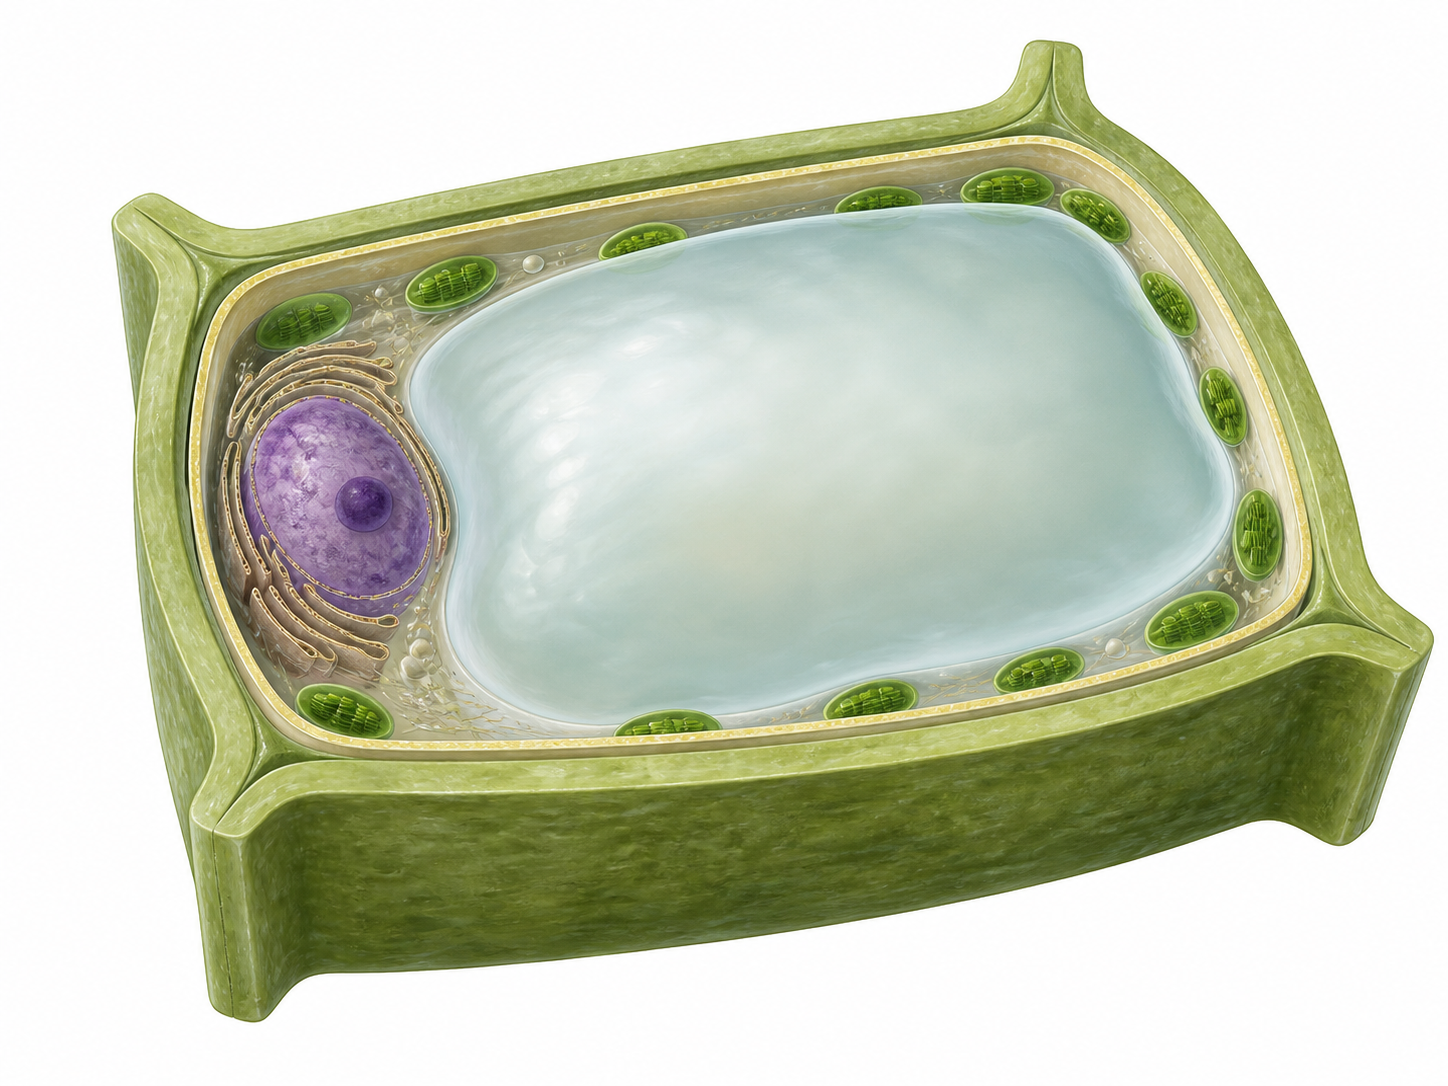
\includegraphics[width=0.98\linewidth]{images/book1/ai/fig-plant-cell.png}};
  \begin{scope}[x={(img.south east)}, y={(img.north west)},
      every node/.style={font=\footnotesize}]
    \draw[omMeth!60!black, thick] (0.16,0.80) -- (0.08,0.94)
      node[above, align=center] {कोशिका\\ भित्ति};
    \draw[omDef, thick] (0.26,0.53) -- (0.22,-0.04)
      node[below] {केंद्रक};
    \draw[omMeth!60!black, thick] (0.72,0.24) -- (0.85,-0.04)
      node[below] {हरे कण};
    \draw[omDef!70, thick] (0.62,0.55) -- (0.70,1.04)
      node[above, align=center] {पानी की\\ थैली};
  \end{scope}
\end{tikzpicture}

{\small पौध \omterm{def:g5:first-look-at-cells:cell}{कोशिका}: वही सामान, और साथ\\ में भित्ति, हरे कण तथा पानी की
थैली}
\end{minipage}

\medskip
{\small दोनों मशहूर \omterm{def:g5:first-look-at-cells:cell}{कोशिकाएँ} अगल-बगल। तीन हिस्सों वाला सामान वही; और
पौध \omterm{def:g5:first-look-at-cells:cell}{कोशिका} उसमें अपनी भित्ति, अपने हरे कण तथा अपनी फूली हुई पानी की
थैली जोड़ लेती है।}
\end{omfigure}

\begin{example}[स्लाइडें अलग पहचानना]\label{ex:g6:cell-unit-of-life:slides}
\cref{ex:g5:first-look-at-cells:classics} की दोनों स्लाइडों के साथ
\omterm{def:g5:first-look-at-cells:microscope}{सूक्ष्मदर्शी} पर लौटो, और अब उन फ़र्क़ों के नाम भी हैं। प्याज़ की \omterm{def:g6:cell-unit-of-life:parts}{झिल्ली}:
कोनों पर मिलती सीधी दीवारें --- यानी \omterm{prop:g6:cell-unit-of-life:plantextras}{कोशिका भित्तियाँ}; और एक तरफ़ खिसका
हुआ \omterm{def:g6:cell-unit-of-life:parts}{केंद्रक} --- यह पानी की थैली की करनी है। गाल की \omterm{def:g5:first-look-at-cells:cell}{कोशिकाएँ}: कोई
भित्ति नहीं, नरम गोल किनारे --- सिर्फ़ \omterm{def:g6:cell-unit-of-life:parts}{झिल्ली} --- और \omterm{def:g6:cell-unit-of-life:parts}{केंद्रक} बीच के
पास। अब एक ही नज़र \omterm{def:g1:plants-around-us:plant}{पौधा} या \omterm{def:g1:animals-around-us:animal}{जंतु} पढ़ लेती है।
\end{example}

\section{एक ही कोशिका में पूरे जीवन}

\begin{definition}[एककोशिकीय सजीव]\label{def:g6:cell-unit-of-life:unicellular}
\emph{एककोशिकीय}\index{एककोशिकीय} \omterm{def:g6:exploring-our-environment:components}{सजीव} ठीक एक ही \omterm{def:g5:first-look-at-cells:cell}{कोशिका} का पूरा जीव है
(\cref{rem:g5:first-look-at-cells:onecelled})। एक ही \omterm{def:g6:cell-unit-of-life:parts}{झिल्ली} के भीतर वह
पोषण लेता है, चलता है, भाँपता है और जनन भी करता है --- दो में बँटकर
(\cref{prop:g5:first-look-at-cells:growth} वाला विभाजन, पर पूरी
जीवन-कथा के रूप में)। \cref{ex:g6:producing-our-food:bread} का \omterm{ex:g6:producing-our-food:bread}{खमीर}
ऐसा ही एक है; और वैसे ही किसी भी तालाब की बूँद के तैराक, तथा \omterm{def:g6:decomposers-and-soil:soil}{मिट्टी},
दही और हाथों के ज़्यादातर सूक्ष्मजीव।
\end{definition}

\begin{example}[तालाब के पानी की एक बूँद, घुमाकर देखी हुई]\label{ex:g6:cell-unit-of-life:drop}
काँच-घर की हरी दीवार से ली गई एक बूँद, लेंस के नीचे: चप्पू जैसे बालों
से खेती हुई एक चप्पल-नुमा \omterm{def:g5:first-look-at-cells:cell}{कोशिका}, जो नज़र में सबसे तेज़ है; हरी अकेली
\omterm{def:g5:first-look-at-cells:cell}{कोशिकाएँ} --- यानी तैरते \omterm{def:g5:food-webs:roles}{उत्पादक}, जो किसी भी \omterm{def:g1:plants-around-us:parts}{पत्ती} की तरह \omterm{def:g6:exploring-our-environment:conditions}{प्रकाश} पकड़ते
हैं; और एक लोंदा, जो अपने भोजन के चारों ओर बहकर उसे पूरा निगल लेता है।
इनमें से हर एक पोषण ले रहा है, चल रहा है, बच रहा है --- यानी किसी
\omterm{def:g1:animals-around-us:animal}{जंतु} या \omterm{def:g1:plants-around-us:plant}{पौधे} का पूरा जीवन, एक ही \omterm{def:g5:first-look-at-cells:cell}{कोशिका} के बजट में।
\end{example}

\begin{remark}[एक कोशिका या कई: जीने के दो ढंग]\label{rem:g6:cell-unit-of-life:twoways}
\omterm{def:g6:cell-unit-of-life:unicellular}{एककोशिकीय} जीव सब कुछ एक ही \omterm{def:g5:first-look-at-cells:cell}{कोशिका} से करता है; तुम्हारा शरीर सब कुछ
दसियों हज़ार अरब \omterm{def:g5:first-look-at-cells:cell}{कोशिकाओं} से करता है, और वे \emph{विशेषज्ञ} होती हैं
--- अस्तर के लिए गाल की \omterm{def:g5:first-look-at-cells:cell}{कोशिकाएँ}, \omterm{def:g3:bones-and-muscles:muscle}{संकुचित} होने वाली \omterm{def:g3:bones-and-muscles:muscle}{पेशी} \omterm{def:g5:first-look-at-cells:cell}{कोशिकाएँ}
(\cref{def:g3:bones-and-muscles:muscle}), और
\cref{prop:g5:brain-in-command:loop} के संदेश ढोने वाली \omterm{def:g5:brain-in-command:system}{तंत्रिका}
\omterm{def:g5:first-look-at-cells:cell}{कोशिकाएँ}। कई \omterm{def:g5:first-look-at-cells:cell}{कोशिकाएँ} काम के बँटवारे की छूट देती हैं; और एक \omterm{def:g5:first-look-at-cells:cell}{कोशिका} का
मतलब है हर पेशा एक ही कमरे में। दोनों योजनाएँ चलती हैं: धरती पर सबसे
ज़्यादा संख्या \omterm{def:g6:cell-unit-of-life:unicellular}{एककोशिकीय} जीवों की ही है।
\end{remark}

\section{कोशिका सिद्धांत}

\begin{proposition}[कोशिका सिद्धांत]\label{prop:g6:cell-unit-of-life:theory}
सदियों में बने दो वाक्य इस अध्याय और
\cref{ch:g5:first-look-at-cells} का सार कह देते हैं:
\begin{enumerate}
  \item हर \omterm{def:g6:exploring-our-environment:components}{सजीव} एक या एक से ज़्यादा \omterm{def:g5:first-look-at-cells:cell}{कोशिकाओं} से बना है, और \omterm{def:g5:first-look-at-cells:cell}{कोशिकाएँ} ही
        जीवन की सबसे छोटी इकाइयाँ हैं;
  \item और हर \omterm{def:g5:first-look-at-cells:cell}{कोशिका} किसी पहले से मौजूद \omterm{def:g5:first-look-at-cells:cell}{कोशिका} के विभाजन से ही आती
        है।
\end{enumerate}
इनका कोई अपवाद कभी नहीं मिला --- न सबसे गहरे समुद्र में, न सबसे पुराने
चट्टानी कुंड में। दूसरे वाक्य का एक बहुत बड़ा नतीजा है: आज जीवित हर
\omterm{def:g5:first-look-at-cells:cell}{कोशिका} विभाजनों की एक अटूट शृंखला आगे बढ़ा रही है जो शुरुआती जीवन तक
पीछे जाती है --- यानी \omterm{prop:g6:classification-kinship:kinship}{नातेदारी}
(\cref{prop:g6:classification-kinship:kinship}), \omterm{def:g5:first-look-at-cells:cell}{कोशिका} के पैमाने पर
लिखी हुई।
\end{proposition}
\admitted

\begin{method}[किसी भी जीव को कोशिका के पैमाने पर पढ़ना]\label{met:g6:cell-unit-of-life:read}
कोई भी \omterm{def:g6:exploring-our-environment:components}{सजीव} सामने हो, तो:
\begin{enumerate}
  \item पहले पूछो: एक \omterm{def:g5:first-look-at-cells:cell}{कोशिका}, या कई?
  \item अगर कई हैं: तो विशेषज्ञ क़िस्मों की उम्मीद करो --- अस्तर बनाने
        वाली, ढोने वाली, \omterm{def:g3:bones-and-muscles:muscle}{संकुचित} होने वाली, कमान चलाने वाली;
  \item \omterm{def:g1:plants-around-us:plant}{पौधा} या \omterm{def:g1:animals-around-us:animal}{जंतु}? \omterm{def:g5:first-look-at-cells:microscope}{सूक्ष्मदर्शी} पर भित्तियाँ और हरे कण जाँचो;
  \item और जो भी वृद्धि, मरम्मत या जनन तुम देखो: उसे \omterm{def:g5:first-look-at-cells:cell}{कोशिकाओं} के
        विभाजनों में अनुवाद करो --- दूसरा वाक्य गारंटी देता है कि यह
        अनुवाद मौजूद है।
\end{enumerate}
\end{method}

\begin{example}[यह सिद्धांत इस पुस्तक में काम पर]\label{ex:g6:cell-unit-of-life:atwork}
पहले वाक्य ने \omterm{prop:g5:first-look-at-cells:principle}{जीवन की एकता} को आधार दिया
(\cref{prop:g5:first-look-at-cells:principle}); और दूसरे वाक्य ने
विभाजन से वृद्धि को (\cref{ex:g5:first-look-at-cells:one}), गूँधे हुए
आटे में \omterm{ex:g6:producing-our-food:bread}{खमीर} के दुगुने होने को, गरम ढेर में अपघटकों के बढ़ने को, और
\cref{ch:g6:producing-our-food} के सूक्ष्मजीव-कार्यबलों को। एक छोटा-सा
सिद्धांत, जो इस साल के \omterm{def:g1:living-or-not:living}{जीवविज्ञान} का बड़ा हिस्सा उठाए हुए है।
\end{example}

\section{अभ्यास}

\begin{exercise}[$\star$]\label{exo:g6:cell-unit-of-life:1}
हर \omterm{def:g5:first-look-at-cells:cell}{कोशिका} के तीन हिस्सों वाले सामान के नाम बताओ, और हर हिस्से का काम
भी।
\end{exercise}

\begin{exercise}[$\star$]\label{exo:g6:cell-unit-of-life:2}
पौध \omterm{def:g5:first-look-at-cells:cell}{कोशिका} की तीनों अतिरिक्त चीज़ें और हर एक का काम बताओ।
\end{exercise}

\begin{exercise}[$\star$]\label{exo:g6:cell-unit-of-life:3}
\omterm{def:g5:first-look-at-cells:microscope}{सूक्ष्मदर्शी} पर तुम प्याज़ की \omterm{def:g6:cell-unit-of-life:parts}{झिल्ली} की \omterm{def:g5:first-look-at-cells:cell}{कोशिका} को गाल की \omterm{def:g5:first-look-at-cells:cell}{कोशिका} से कैसे
अलग पहचानोगे? दो दिखने वाले फ़र्क़ बताओ।
\end{exercise}

\begin{exercise}[$\star$]\label{exo:g6:cell-unit-of-life:4}
\omterm{def:g6:cell-unit-of-life:unicellular}{एककोशिकीय} \omterm{def:g6:exploring-our-environment:components}{सजीव} क्या है? इस अध्याय से दो के नाम बताओ।
\end{exercise}

\begin{exercise}[$\star$]\label{exo:g6:cell-unit-of-life:5}
\omterm{def:g5:first-look-at-cells:cell}{कोशिका} सिद्धांत के दोनों वाक्य बताओ।
\end{exercise}

\begin{exercise}[$\star$]\label{exo:g6:cell-unit-of-life:6}
\omterm{def:g6:cell-unit-of-life:unicellular}{एककोशिकीय} जीव जनन कैसे करता है?
\end{exercise}

\begin{exercise}[$\star\star$]\label{exo:g6:cell-unit-of-life:7}
\omterm{def:g1:plants-around-us:plant}{पौधे} \omterm{def:g3:bones-and-muscles:skeleton}{हड्डियों} के बिना खड़े कैसे रहते हैं? पौध \omterm{def:g5:first-look-at-cells:cell}{कोशिका} के कौन-से दो
साज़-सामान यह काम बाँटते हैं --- और \omterm{def:g5:first-look-at-cells:cell}{कोशिका} के पैमाने पर मुरझाना क्या
है?
\end{exercise}

\begin{exercise}[$\star\star$]\label{exo:g6:cell-unit-of-life:8}
\cref{prop:g6:plants-are-producers:produce} की \omterm{def:g5:food-webs:roles}{उत्पादकों} वाली कार्यशाला
\omterm{def:g5:first-look-at-cells:cell}{कोशिका} का कौन-सा हिस्सा है? और
\cref{prop:g6:matter-from-food:transform} के अनुसार हर \omterm{def:g1:animals-around-us:animal}{जंतु} \omterm{def:g5:first-look-at-cells:cell}{कोशिका} में
उसका न होना ज़रूरी क्यों है?
\end{exercise}

\begin{exercise}[$\star\star$]\label{exo:g6:cell-unit-of-life:9}
\cref{rem:g6:cell-unit-of-life:twoways} से अपने शरीर की तीन विशेषज्ञ
कोशिका-क़िस्में और हर एक का पेशा बताओ।
\end{exercise}

\begin{exercise}[$\star\star$]\label{exo:g6:cell-unit-of-life:10}
\cref{met:g6:cell-unit-of-life:read} के अनुसार इन्हें कोशिका-विभाजनों
में अनुवाद करो: भरता हुआ छिला \omterm{def:g1:my-body:joint}{घुटना}; रात भर में दुगुना होता आटा; और
बढ़ता हुआ \omterm{ex:g2:animals-grow-up:frog}{टैडपोल}।
\end{exercise}

\begin{exercise}[$\star\star$]\label{exo:g6:cell-unit-of-life:11}
तालाब की बूँद के हरे तैराक अकेली \omterm{def:g5:first-look-at-cells:cell}{कोशिकाएँ} हैं जो \omterm{def:g6:exploring-our-environment:conditions}{प्रकाश} पकड़ती हैं।
\cref{def:g5:food-webs:roles} का कौन-सा पेशा वे चलाती हैं, और इससे वे
तालाब के \omterm{def:g5:food-webs:web}{आहार जाल} में क्या बन जाती हैं?
\end{exercise}

\begin{exercise}[$\star\star\star$]\label{exo:g6:cell-unit-of-life:12}
\omterm{def:g5:first-look-at-cells:cell}{कोशिका} सिद्धांत के दूसरे वाक्य को उतनी ही गंभीरता से लो जितनी
\cref{rem:g6:classification-kinship:implies} ने \omterm{def:g6:classification-kinship:tree}{वृक्ष} को ली थी:
तुम्हारे गाल की किसी एक \omterm{def:g5:first-look-at-cells:cell}{कोशिका} को दूर के अतीत से कौन-सी अटूट शृंखला
जोड़ती है? इसका नतीजा एक वाक्य में लिखो।
\end{exercise}

\section{समस्या: सूक्ष्मदर्शी वाली दोपहर}

\begin{problem}[{सप्ताहांत समस्या --- चार स्लाइडें, एक
सिद्धांत}]\label{pb:g6:cell-unit-of-life:1}
कक्षा की \omterm{def:g5:first-look-at-cells:microscope}{सूक्ष्मदर्शी} वाली दोपहर: चार पड़ाव, चार स्लाइडें --- प्याज़ की
\omterm{def:g6:cell-unit-of-life:parts}{झिल्ली} (क), गाल की खुरचन (ख), तालाब के पानी की एक बूँद (ग), और दही का
एक लेप (घ)। हर टोली चारों पड़ावों का चक्कर लगाती है और चित्र बनाती
जाती है।

\medskip\noindent\textbf{भाग I --- पड़ाव क और ख।}
\begin{enumerate}
  \item पड़ाव क पर टोली सीधी दीवारों वाली ``ईंटें'' बनाती है, और हर एक
        में एक गहरा धब्बा एक तरफ़ दबा हुआ है। उस दीवार, उस धब्बे, और
        उसे किनारे दबाने वाले अपराधी के नाम बताओ।
  \item पड़ाव ख पर: गोल \omterm{def:g5:first-look-at-cells:cell}{कोशिकाएँ}, कोई दीवार नहीं, और धब्बे बीच में।
        बताओ कि क की \omterm{def:g5:first-look-at-cells:cell}{कोशिकाओं} के पास कौन-सा साज़-सामान है जो ख की
        \omterm{def:g5:first-look-at-cells:cell}{कोशिकाओं} के पास नहीं --- और वह सामान भी जो दोनों साझा करती
        हैं।
  \item एक साथी पूछता है कि ज़मीन के नीचे उगे \omterm{ex:g4:plants-without-seeds:bulbtuber}{शल्ककंद} से ली गई प्याज़ की
        \omterm{def:g5:first-look-at-cells:cell}{कोशिकाओं} में हरे कण क्यों नहीं दिखते। उन कणों के काम और
        \omterm{ex:g4:plants-without-seeds:bulbtuber}{शल्ककंद} के पते से उत्तर दो।
  \item स्लाइड ख पर किसकी \omterm{def:g5:first-look-at-cells:cell}{कोशिकाएँ} हैं? बताओ कि \omterm{def:g5:first-look-at-cells:cell}{कोशिका} सिद्धांत के
        दूसरे वाक्य से इसका क्या निहितार्थ है: उनमें से हर \omterm{def:g5:first-look-at-cells:cell}{कोशिका} आई
        कहाँ से?
\end{enumerate}

\medskip\noindent\textbf{भाग II --- पड़ाव ग और घ।}
\begin{enumerate}[resume]
  \item पड़ाव ग: चप्पल-नुमा खेने वाली, हरे तैराक, और बहता हुआ लोंदा।
        हर एक के लिए बताओ कि मिनट भर देखने में जीवन की कौन-सी
        गतिविधियाँ दिखती हैं --- और फिर निष्कर्ष निकालो कि हर एक है
        क्या।
  \item हरे तैराक अकेली \omterm{def:g5:first-look-at-cells:cell}{कोशिकाएँ} हैं, फिर भी \omterm{def:g5:food-webs:roles}{उत्पादक} हैं। यह साबित करने
        के लिए चित्र में कौन-सा साज़-सामान दिखना ही चाहिए?
  \item पड़ाव घ के दही के लेप में बहुत बड़ी संख्या में जोड़ियों और
        ज़ंजीरों में बँधी नन्ही \omterm{def:g5:first-look-at-cells:cell}{कोशिकाएँ} दिखती हैं। इन्हें
        \cref{ex:g6:producing-our-food:yogurt} से जोड़ो: इन \omterm{def:g5:first-look-at-cells:cell}{कोशिकाओं} ने
        \omterm{def:g2:animals-grow-up:born}{दूध} का क्या किया, और इस अध्याय की शब्दावली में वे हैं क्या?
  \item एक टोली दावा करती है कि स्लाइड घ में ``कोई \omterm{def:g6:exploring-our-environment:components}{सजीव} नहीं, बस कण
        हैं''। धीरज या गरम स्लाइड मिल जाए तो कौन-सा एक प्रेक्षण \omterm{def:g5:first-look-at-cells:cell}{कोशिका}
        सिद्धांत के दूसरे वाक्य से तय कर देगा कि वे कण जीवित हैं या
        नहीं?
\end{enumerate}

\medskip\noindent\textbf{भाग III --- लिखना।}
\begin{enumerate}[resume]
  \item लिखते समय चारों स्लाइडों को इस आधार पर छाँटना है: एक \omterm{def:g5:first-look-at-cells:cell}{कोशिका} या
        कई? \omterm{def:g1:plants-around-us:plant}{पौधा}, \omterm{def:g1:animals-around-us:animal}{जंतु}, या इनमें से कोई नहीं? यह करो।
  \item उस दोपहर का हर चित्र वही तीन हिस्सों वाला सामान दिखाता है। वह
        सामान बताओ, और यह भी कि उसका सब जगह मिलना किस बात का सबूत है
        (\cref{prop:g5:first-look-at-cells:principle})।
  \item शिक्षक अंत में कहते हैं: ``आज तुमने जो कुछ भी बनाया, वह कभी एक
        ही \omterm{def:g5:first-look-at-cells:cell}{कोशिका} था।'' इस वाक्य का बचाव प्याज़ के लिए, गाल की
        \omterm{def:g5:first-look-at-cells:cell}{कोशिकाओं} के मालिक के लिए, और दही की ज़ंजीरों के लिए करो।
  \item उस दोपहर के निष्कर्ष को \omterm{def:g5:first-look-at-cells:cell}{कोशिका} सिद्धांत के रूप में --- दो
        वाक्यों में --- लिखो, और हर स्लाइड के लिए यह भी बताओ कि उसने
        कौन-सा वाक्य सबसे अच्छी तरह दिखाया।
\end{enumerate}
\end{problem}
